%!TEX root = ../MasterThesis.tex

\section{Stakeholder Analysis}
\label{sec:stakeholder_analysis}

The following section will look at each stakeholder involved in detail and lists  the kind of information they have at hand.

\subsection{Consumer}
\label{subsec:stakeholder_consumer}

The \textbf{consumer} is the initiator of an E-commerce transaction. She is using the shop of a \textbf{merchant} on the Internet to order products or services. For doing so she has to know the \gls{URL} of the Web shop, has to be connected to the Internet via the \textbf{\gls{ISP}} and has to use a standard software called a Web Browser on her computer. For the duration of her online session she receives an unique \textbf{\gls{IP}} address from the \gls{ISP}.\\

She might have had a long-term business relationship with the merchant and already owns an \textbf{user account} on the Web shop. On the other hand she might be just interested into a one-time shopping trip and might want to order the items without creating an account first --- sometimes also called ``anonymous shopping'' in the E-commerce scenario. \\

The consumer is also having a \textbf{bank account} and at least owns a \textbf{debit card} with the \textbf{issuing bank} to get access to the money on that account. In addition to that she can also hold multipe \textbf{credit cards}. A credit card can be issued by the same bank or can be provided by other financial services (e.g. American Express). In any case the organisation that has handed out the credit card to the consumer is called the \textbf{issuer}. \\

If she is going to order items in a Web shop, she will usually browse the product and service offerings of the merchant first and put the articles of interest into the \textbf{shopping cart}. When finalizing the transaction she has to hand over the following information to the merchant:\@

\begin{itemize}
		\item personal information incl. given name, family name and date of birth
		\item the address the items should be shipped to
		\item payment information incl. type of payment and billing address (if different to shipping address)
\end{itemize}

If she is going to end the transaction with a payment of type \textbf{credit card} she will have to provide the specific information of the card to be used:\@

\begin{itemize}
		\item credit card owner
		\item credit card number
		\item credit card expiry date (in format MM/YY)
		\item credit card security code
\end{itemize}

The consumer is having a special role in the whole scenario. As the merchant has to deal with the consumer without any face-to-face or real-world interaction, the consumer is also the less thrustworthy party from the point of view of the merchant. As the Section~\ref{sec:scenario_fraud} will show the consumer is the main object of question in the case of an E-commer fraud. For the investigation of it the consumer is usually not taking an active part.

% subsection stakeholder consumer

\subsection{Merchant}
\label{subsec:stakeholder_merchant}

The \textbf{merchant} offers products and services on the Internet for the general public. She might use the Internet as an additional sales channel or rely on it solely for making any business. To provide access to the \textbf{Web shop} the merchant has to register a domain name and \textbf{\gls{URL}} at a local domain name registry. This specific \gls{URL} refers to a fixed public \gls{IP} address, that the server hosting the Web shop software uses. Normally the merchant does not run the servers herself, but rely on a service offering from a hosting or \textbf{cloud service provider} for that. Also the Web shop software itself is usually not provided by the merchant, but bought from an \textbf{\gls{ISV}} on the market. In any case the merchant has special rights in the Web shop as she is allowed to configure the products, prices, promotions, available payment and shipment services. In addition products can be categorized into departments and sub-departments for easier navigation in the online shop. \\

The merchant can decide whether she restricts ordering of products to registered users only, or allows anonymous users too. The main benefit of the former is the possibility to analyse the \textbf{shopping behaviour} of individual consumers, whereas the latter will open the business for a wider range of consumers as it includes also those, that do not want to register with any online shop. Nevertheless any consumer activity on the online shop is traced in the analytic databases of the merchant. This includes not only the items, that have been placed into the shopping cart, but also any product that has been looked at during a shopping session. Even if these detailed analytic capabilities are actually synonymous for their usage in target-related advertising, they can also help to decide if a consumer behaves normally or not. \\

Any business transaction that the consumer makes with the merchant is stored in the merchant's databases. A transaction information contains, but is not limited to:\@

\begin{itemize}
		\item the personal information of the consumer
		\item the address the items will be shipped to
		\item a collection of products with quantities and prices
		\item the total amount of the order considering promotions, taxes and fees
		\item the selected payment information
\end{itemize}

If the consumer pays with credit card the merchant do not handle the payment herself, but relate this action to a \textbf{Payment Service Provider}. In return of the payment authorization the merchant will receive and store the following payment-related information for the transaction:\@

\begin{itemize}
		\item the type of credit card used (e.g. Visa, MasterCard, American Express, \ldots)
		\item the credit card information incl. credit card number, expiry date and security code
		\item the name of the credit card owner
		\item the payment token received by the \gls{PSP}
		\item the timestamp and result code of the authorization
		\item the authority who approved the payment (if the merchant works with multiple Payment Service Providers)
\end{itemize}

As a merchant will collect a lot of personal and payment related information over time, she is also one of the major sources of possible data leaks in this scenario. Based on this fact the Payment Card Initiative, a group of banks, issuers and \gls{PSP}s, provides rules and guidelines (aka PCI/DSS standards) for securely handling these kinds of information in an IT system \citep{dss2014payment}. \\

A merchant is one of the main actors in the fraud investigation process. She is interested in figuring out whether the consumer's transaction is valid or not. As in a case of an E-commerce fraud the merchant will mostly have to cover the costs of the incident (see Section~\ref{sec:scenario_fraud}). Also the online merchant's reputation will suffer, if private information from her databases get leacked. If a merchant falls victim to a fraud incident multiple times, the economic damages can finally result in a bankruptcy of the merchant.

% subsection stakeholder merchant

\subsection{Payment Service Provider}
\label{subsec:stakeholder_psp}

The \textbf{Payment Service Provider} is offering payment-related services to online merchants. As of this the \gls{PSP} provides a common Web interface, that the merchant has to communicate with for sending payment authorization requests. The \gls{PSP} might be able to authorize the payment request on her own or have to route the request to the corresponding \textbf{issuer} of the credit card in question. For the former procedure the \gls{PSP} has to run an own database of registered users with their credit card information (e.g. PayPal). For checking the credit card and authorizing the payment the \textbf{merchant} is sending the following information from the transaction:\@

\begin{itemize}
		\item credit card owner
		\item credit card number
		\item credit card expiry date
		\item credit card security number
		\item identification of the merchant
		\item current transaction total amount
\end{itemize}

The \gls{PSP} has to securely process these information and return the result of the examination to the merchant. The result message also contains an unique payment token, that the merchant can refer to later to initiate the clearing process. As of this the \gls{PSP} have to persist the credit card and transaction related information in her own backend databases. Following industry standards she should do so according to the PCI/DSS guidelines mentioned above.\\

The level of activity in the E-commerce fraud investigation process depends on whether the \gls{PSP} authorizes the payment herself or only acts as routing service between the merchant and the original credit card issuer. In the former case the \gls{PSP} is more actively involved. In that case she also holds more of the valuable information to solve the incident. In the latter case she might be able to connect the payment-related request information from the merchant with the authorization result coming from the issuer.\\

If the \gls{PSP} holds sensitive information in her own databases she might also be a source of data leaks. In that case she should make the same precautions as an issuing bank will have to do.

% subsection stakeholder psp

\subsection{Issuing Bank}
\label{subsec:stakeholder_issuer}

The \textbf{issuer} is one of the parties in the scenario that knows the owner of the credit card in person. Each individual has to register personally with the issuer to get access to a credit card. This includes providing the following information:\@

\begin{itemize}
		\item personal information like given name, family name and date of birth
		\item the current home address
		\item the bank account that should be used to settle credit card balances
\end{itemize}

Even if the two parties do not really meet each other personally, a person will still have to identify with a valid id card and bank account to receive and activate a new credit card. Beside being the single source of truth about the original credit card owner, the issuer of the card also collects and stores all  usages of it. The issuer therefore can provide credit card usage patterns, that are not just limited to the online shopping scenario --- something a Payment Service Provider might also be able to deliver; but also include transactions the card owner does in the real-world. Needless to say that these are valuable information for the E-commerce fraud investigation. \\

Still the issuer does not know the details of the transactions, that have been made with the credit card. As mentioned above in the section about the \gls{PSP} the issuer will just receive an identifier of the merchant, in whose shop the credit card has been used. Based on public available information of the merchant from a commercial register, the issuer could at least come up with the retail branch the merchant belongs to. \\

Being the single source of truth about all issued credit cards and their owners the issuer is another high-risk for data leaks. She should as well follow the guidelines from the PCI/DSS standards and monitor her backend systems heavily with an intrusion detection mechanism.

% subsection stakeholer issuer

\subsection{Acquiring Bank}
\label{subsec:stakeholder_acquirer}

The \textbf{acquirer} holds the bank account of the merchant and is responsible for withdrawing the outstanding amounts of transactions from the accounts of the consumers, or more precisely the issuing bank of each consumer. As of this the acquiring bank is usually not processing any credit card related information from consumers, but refer to the payment tokens that have been given by the \gls{PSP} or issuer during the authorization process. \\

Still as a financial institute the acquirer has to comply with the rules and guidelines of the PCI/DSS and other industry standards to make sure, that her bank accounts and the transaction processing are safe and secure. The detailed analysis of these procedures and their possible (banking) frauds are out of scope of this thesis though.

% subsection stakeholder acquirer

\subsection{Logistic Service Provider}
\label{subsec:stakeholder_lsp}

The \textbf{Logistic Service Provider} has two important roles in the E-commerce scenario. First she has access to and control over the items of the merchant for the duration of the transport between the merchant's facility and the consumer's shipping address. And second she holds the information to whom she has handed over the items at the final destination. Although the \gls{LSP} has nothing to do with any payment related activities, she might be the last chance for the merchant to stop the delivery of the items (in case a fraud has been detected after shipment) or provide information about the person, that has received the items at the shipping address --- especially on high-priced goods, which usually require the recipient to show her personal id card and place a signature on the delivery receipt. \\

For initiating the shipment procedure the merchant is ordering a certain transport service from the \gls{LSP} and hand over the following information:\@

\begin{itemize}
	\item name of the receiver
	\item delivery address
	\item list of items to be shipped
	\item optionally: value of the items if an insurance policy is taken
\end{itemize}

The \gls{LSP} at the other hand returns an unique \textbf{tracking id} for the shipment. It can be used by the merchant and the consumer to check the status of the shipment online. \\

As the \gls{LSP} does not have to deal with the payment related activities in the E-commerce scenario, she is also not actively involved in the fraud investigation. Still she is of help if an incident is found as she can stop the delivery or provide the information of the recipient.

% subsection stakeholder lsp

\subsection{Cloud Service Provider}
\label{subsec:stakeholder_csp}

The \textbf{Cloud Service Provider} offers IT services to its customers. These IT services include hardware and software assets, that in the E-commerce scenario a merchant can order to run her Web shop on the Internet. Part of the service level agreement between the merchant and the \gls{CSP} is a detailed listing of the responsibilities of both parties (who has to take care of what). In most cases the merchant is outsourcing the complete operation of the hardware and software for the Web shop to the \gls{CSP}; so the \gls{CSP} would be responsible for making sure the Web shop is available and secure. The \gls{CSP} is also constantly monitoring the incoming connections to each public Internet server under her control and might provide information, whether a Web shop of one of the merchants using the services of the \gls{CSP} has been compromised or not.

% subsection stakeholder csp

\subsection{Independent Software Vendor}
\label{subsec:stakeholder_isv}

The \textbf{ISV} designs, implements and sells the Web shop software. She has detailed knowledge about the software components and libraries used within the Web shop and normally also monitors them for security breaches or vulnerabilities. She also has to verify the software code implemented on her own for vulnerabilities, and additionally has to make sure that the implementation follows industry standards (e.g. PCI/DSS for handling person and payment related information). As of this she can best assert these quality criterias of the Web shop if needed.

% subsection stakeholder isv

\subsection{Internet Service Provider}
\label{subsec:stakeholder_isp}

The \textbf{ISP} provides a service to the consumer for connecting to the Internet. Each Web request the consumer is doing on her system is routed to the public Internet via the infrastructure of the \gls{ISP}. Due to regulations and laws the \gls{ISP} has to store the log files of any Internet session of its customers for a certain amount of time. Especially these log files can be helpful to decide whether a consumer was visiting pages in the dark-side of the Web, or if she falls victim to some phishing attacks (explained later in Section~\ref{sec:scenario_fraud}).

% subsection stakeholder isp

\subsection{Data Flow}
\label{subsec:stakeholder_data_flow}

The flow of data between the important stakeholders involved in the scenario of credit card frauds in E-commerce is shown in Figure~\ref{fig:images_e_commerce_stakeholder}. \@

\begin{figure}[H]
	\centering
		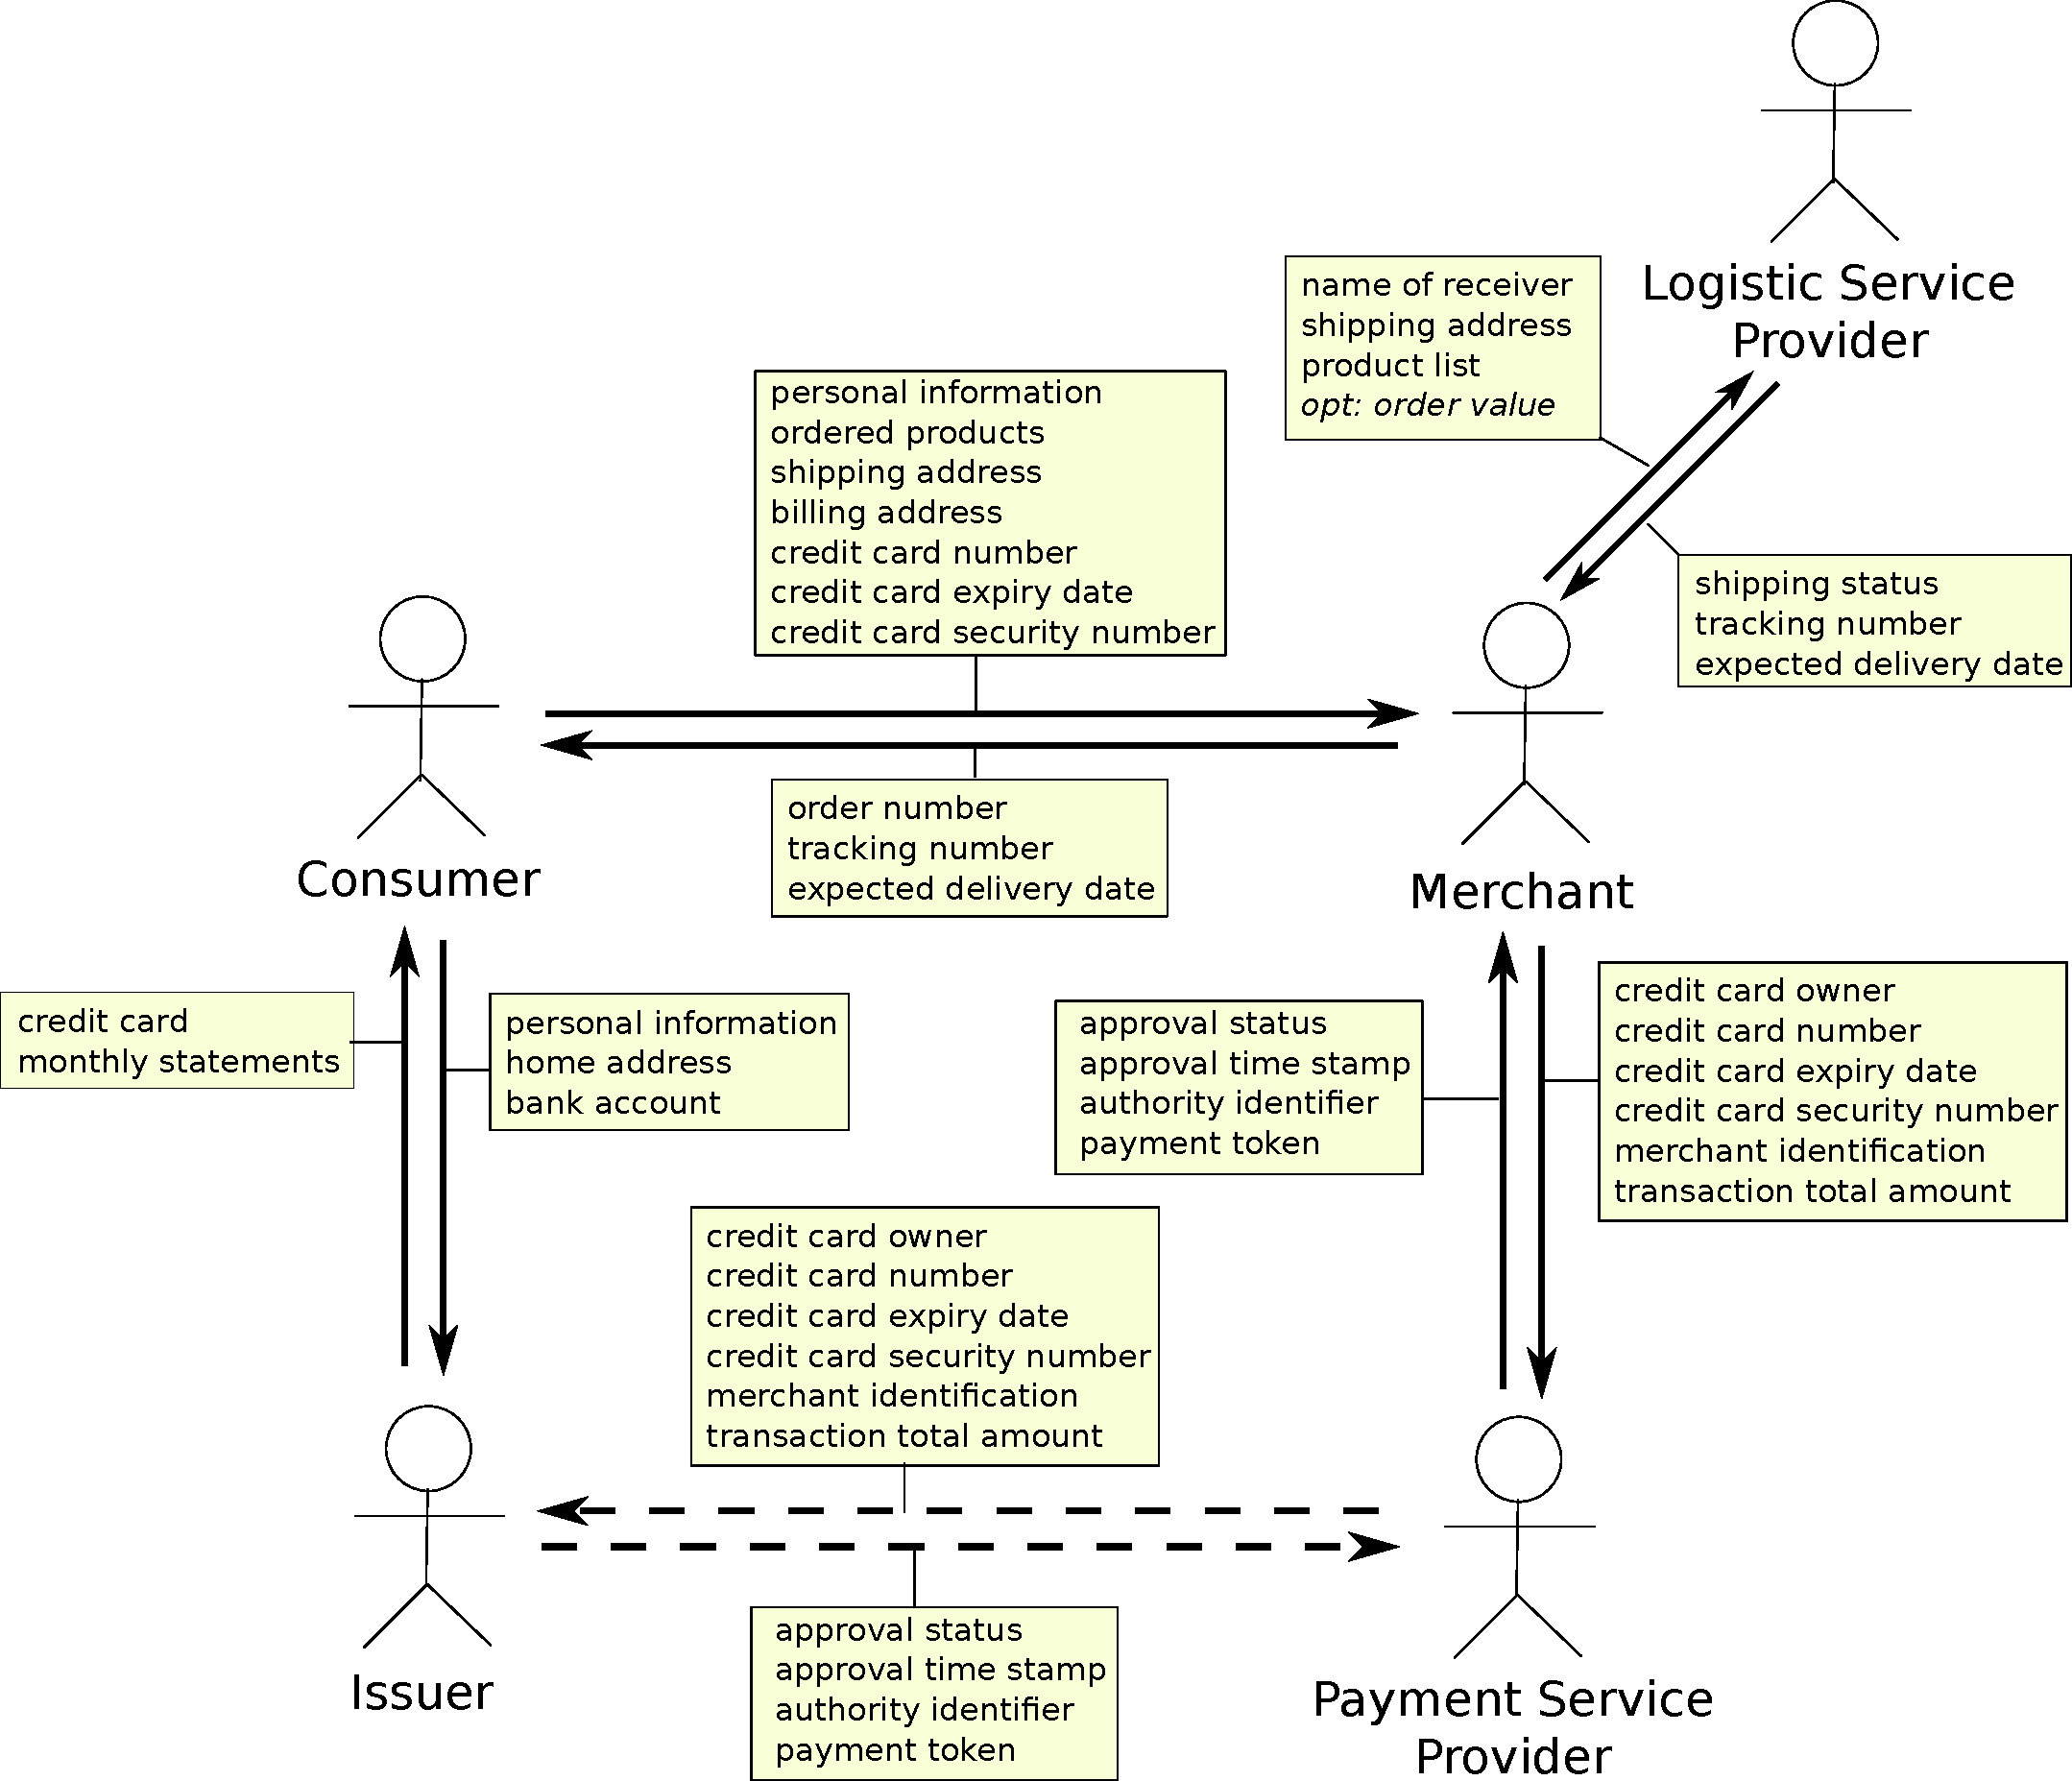
\includegraphics[width=0.8\columnwidth]{images/e-commerce-stakeholder.pdf}
	\caption{Stakeholder and Data Flow in E-commerce scenario}
\label{fig:images_e_commerce_stakeholder}
\end{figure}


% section stakeholder analysis
